\begin{frame}[fragile]{Visualização da representação por matriz de adjacências}

    \begin{figure}
        \centering

        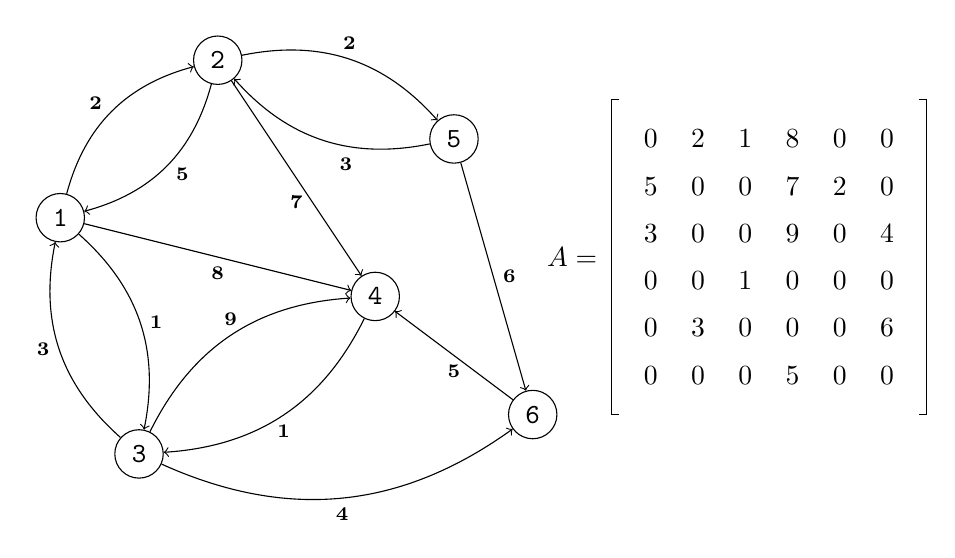
\begin{tikzpicture}
            \node[draw,circle] (A) at (0, 3) { \tt 1 };
            \node[draw,circle] (B) at (2, 5) { \tt 2 };
            \node[draw,circle] (C) at (1, 0) { \tt 3 };
            \node[draw,circle] (D) at (4, 2) { \tt 4 };
            \node[draw,circle] (E) at (5, 4) { \tt 5 };
            \node[draw,circle] (F) at (6, 0.5) { \tt 6 };

            \draw[->] (A) to [bend left] node[anchor=east,yshift=0.1cm] { \scriptsize $\mathbf{2}$ } (B);
            \draw[->] (B) to [bend left] node[anchor=west,yshift=-0.1cm] { \scriptsize $\mathbf{5}$ } (A);
            \draw[->] (A) to [bend left] node[anchor=west] { \scriptsize $\mathbf{1}$ } (C);
            \draw[->] (C) to [bend left] node[anchor=east] { \scriptsize $\mathbf{3}$ } (A);
            \draw[->] (D) to [bend left] node[anchor=north] { \scriptsize $\mathbf{1}$ } (C);
            \draw[->] (C) to [bend left] node[anchor=south] { \scriptsize $\mathbf{9}$ } (D);
            \draw[->] (B) to [bend left] node[anchor=south] { \scriptsize $\mathbf{2}$ } (E);
            \draw[->] (E) to [bend left] node[anchor=north,xshift=0.3cm,yshift=-0.1cm] { \scriptsize $\mathbf{3}$ } (B);

            \draw[->] (A) -- node[anchor=north] { \scriptsize $\mathbf{8}$ } (D);
            \draw[->] (B) -- node[anchor=north,yshift=-0.1cm] { \scriptsize $\mathbf{7}$ } (D);
            \draw[->] (C) to [bend right] node[anchor=north] { \scriptsize $\mathbf{4}$ } (F);
            \draw[<-] (D) -- node[anchor=north] { \scriptsize $\mathbf{5}$ } (F);
            \draw[->] (E) -- node[anchor=west] { \scriptsize $\mathbf{6}$ } (F);

            \node at (6.5, 2.5) { $A = $ };
            \draw (7.1, 4.5) -- (7, 4.5) -- (7, 0.5) -- (7.1, 0.5);
            \draw (10.9, 4.5) -- (11, 4.5) -- (11, 0.5) -- (10.9, 0.5);

            \node at (7.5, 4) { $0$ };
            \node at (8.1, 4) { $2$ };
            \node at (8.7, 4) { $1$ };
            \node at (9.3, 4) { $8$ };
            \node at (9.9, 4) { $0$ };
            \node at (10.5, 4) { $0$ };

            \node at (7.5, 3.4) { $5$ };
            \node at (8.1, 3.4) { $0$ };
            \node at (8.7, 3.4) { $0$ };
            \node at (9.3, 3.4) { $7$ };
            \node at (9.9, 3.4) { $2$ };
            \node at (10.5, 3.4) { $0$ };

            \node at (7.5, 2.8) { $3$ };
            \node at (8.1, 2.8) { $0$ };
            \node at (8.7, 2.8) { $0$ };
            \node at (9.3, 2.8) { $9$ };
            \node at (9.9, 2.8) { $0$ };
            \node at (10.5, 2.8) { $4$ };

            \node at (7.5, 2.2) { $0$ };
            \node at (8.1, 2.2) { $0$ };
            \node at (8.7, 2.2) { $1$ };
            \node at (9.3, 2.2) { $0$ };
            \node at (9.9, 2.2) { $0$ };
            \node at (10.5, 2.2) { $0$ };

            \node at (7.5, 1.6) { $0$ };
            \node at (8.1, 1.6) { $3$ };
            \node at (8.7, 1.6) { $0$ };
            \node at (9.3, 1.6) { $0$ };
            \node at (9.9, 1.6) { $0$ };
            \node at (10.5, 1.6) { $6$ };

            \node at (7.5, 1.0) { $0$ };
            \node at (8.1, 1.0) { $0$ };
            \node at (8.7, 1.0) { $0$ };
            \node at (9.3, 1.0) { $5$ };
            \node at (9.9, 1.0) { $0$ };
            \node at (10.5, 1.0) { $0$ };

        \end{tikzpicture}

    \end{figure}

\end{frame}
